\section{Experiment Overview}
\label{sec:experimental_overview}
\CENTREX\ consists of a series of modules. %each of which perform a different function needed for the measurement.
In this section we describe each region and its function, following the path of a typical TlF molecule in the experiment. A cryogenic buffer gas \emph{beam source} (BS) forms a cold, slow, and bright molecular beam. Next, a \emph{rotational cooling region} (RC) accumulates molecules from the many thermally populated %sublevels
states into a single hyperfine state in $J=0$.
Next, the molecules are coherently transferred from $J=0$ to $J=2,\,m_J=0$ in \emph{state preparation region A} (SPA). This makes it possible to focus the molecular beam at a final detection region downstream with the \emph{electrostatic quadrupole lens} (EQL). \emph{State preparation region B} (SPB) coherently moves population from $J=2,\,m_J=0$ to $J=1,\,m_J=\pm 1$, the states used for the Schiff moment measurement. Next, the \emph{main interaction region} (MI) performs nuclear magnetic resonance (NMR) in the presence of a strong polarizing $\Evec$-field using the technique of separated oscillatory fields (SOF) \cite{PhysRev.78.695,ramsey1951phase}. A short RF magnetic field subregion creates a superposition of thallium nuclear spin states. After a period of free precession in $\Evec$, a second RF field subregion maps the phase accumulation due to the energy difference of the spin states---including a contribution from the Schiff moment---into a population difference between the spin states. In \emph{state preparation region C} (SPC), each spin state is transferred to a different rotational state. Finally, the rotational populations are read out with laser-induced fluorescence (LIF) and optical cycling in the \emph{fluorescence detection region} (FD). An overview of the beamline design is shown in Figures~\ref{fig:beamline} and~\ref{fig:beamline_schematic}.
\begin{figure*}
	\centering
	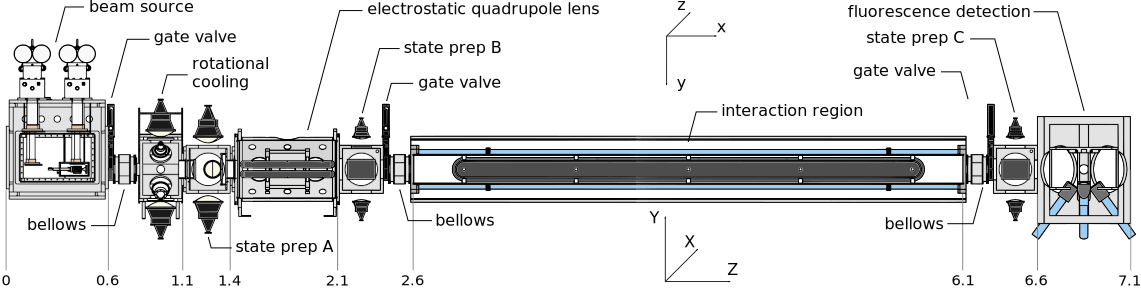
\includegraphics[width=\textwidth]{figs/svg/beamline_v2.pdf}
	\caption{Overview of the planned \CENTREX\ beamline. Distance in meters is shown on the bottom. Modules following the electrostatic quadrupole lens are currently being designed, so few details are given.}
	\label{fig:beamline}
\end{figure*}
\begin{figure*}
	\centering
	\def\svgwidth{\textwidth}
	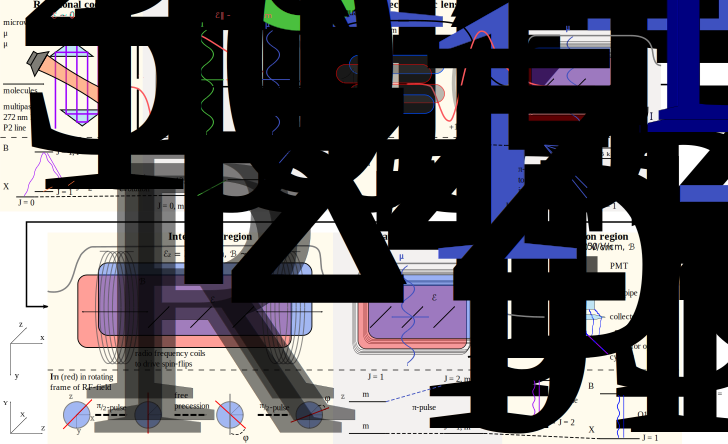
\includegraphics[width=\textwidth]{figs/svg/whole_experiment_A4.pdf}
	\caption{Overview of the regions the TlF molecules traverse as they move through the \CENTREX\ beamline. After emerging from the beam source (not shown), the molecules enter the rotational cooling region. Here, the population in the rotational levels $J = 1$, 2, and 3 is optically pumped to $\ket{J=0,\,F=0}$. (See Sec.~\ref{sec:rotational_cooling} and Fig.~\ref{fig:rotational_cooling_scheme} for more detail.) From there, they move into state preparation region A, where adiabatic passage is applied twice to transfer the molecules to $\ket{J=2,\ m_J=0}$ (Sec.~\ref{sec:state_preparation_region_a}), the state focused by the electrostatic lens (Sec.~\ref{sec:electrostatic_lens}). In state preparation region B (Sec.~\ref{sec:state_preparation_B}), the molecular state is transferred into one of the $\ket{J=1,\ m_J=\pm1}$ states before proceeding to the interaction region (Sec.~\ref{sec:interaction_region}). Here, using NMR with the SOF technique, we transform the frequency shift between Tl spin up and down states, due to $\mathcal{H}_\text{CPV}$ (Eq. \ref{eq:Hamiltonian_effective_interaction}), into a population difference between these states. Subsequently, in state preparation region C (Sec.~\ref{sec:state_preparation_region_c}), one of the Tl spin state populations is transferred to a $J=2$ state. This makes the two populations resolvable with laser-driven transitions, to facilitate state readout (Sec.~\ref{sec:detection_region}). Finally, in the detection region, optical cycling and fluorescence collection are used for efficient, quasi-simultaneous detection of the two populations.  The red, grey, and black curves in the figure indicate the magnitude of the electric field along, respectively, the beam direction $Z$, the interaction region field direction $z$, and the transverse electric quadrupole field directions $X,Y$.}
	\label{fig:beamline_schematic}
\end{figure*}

Because the quantizing fields in \CENTREX~change direction throughout the apparatus, we find it useful to use two different coordinate systems.  We use $(X,Y,Z)$ to denote ``beamline'' coordinates, where $\hat{Z}$ points in the average direction of the molecular beam and $\hat{Y}$ is vertical upward. Similarly, we use $(x,y,z)$ to denote ``interaction region'' coordinates. Here, $\hat{z}$ lies along a line parallel to the average $\Evec$-field in the interaction region, $\langle\Evec\rangle_{\rm MI}$, $\hat{x}$ is the vector closest to the average beam velocity that is also perpendicular to $\hat{z}$, and $\hat{y}$ is the vector closest to downward (along gravity) that is perpendicular to $\hat{z}$ and $\hat{x}$.  
The direction of $\hat{z}$ (parallel or antiparallel to $\langle\Evec\rangle_{\rm MI}$) is fixed in the lab, set by the definitions of $\hat{x}$ and $\hat{y}$ and by demanding a right-handed coordinate system.  Hence, the $\Evec$ field in the MI region is (nominally) $\Evec = \Esca \hat{z}$, where $\Esca$ can take either sign.

\subsection{Beam Source}
\label{sec:beamsource}
The source of the TlF molecules is a cryogenic neon buffer gas beam \cite{hutzler2012buffer}. A copper cell containing a solid TlF target is cooled to $18\,$K. The TlF is ablated with a pulsed Nd:YAG laser operating at up to $50\Hz$, while Ne flows continuously through the cell at a typical rate of $40\sccm$. A $4\kelvin$ layer surrounds the cell and cryopumps the Ne.  Ablated TlF reaches thermal equilibrium with the Ne buffer gas before the cell exit, where the beam cools further as it expands into vacuum. The cold cell aperture ($6.35\mm$ diameter) defines the zero position along the beamline axis, $\vec{Z}$. Two $25.4\mm$ diameter apertures (one in the $4\kelvin$ layer at $Z=43\mm$, one in a blackbody shield at $Z=81\mm$) collimate the beam. 

The velocity distributions of the TlF beam were measured as follows. An additional collimator 
%(rectangular, $2\times 5.4$ mm$^2$) 
was placed downstream. After this collimator, a laser beam, tuned to a $Q1$ line of the $X-B$ transition, crossed the molecular beam. Here, laser-induced fluorescence (LIF) was recorded with a photomultiplier tube (PMT). The LIF signal as a function of laser detuning, with laser beams perpendicular to or at $45^\circ$ to the TlF beam, yielded information on the velocity distributions. The longitudinal distribution is very nearly Gaussian, with mean $\langle v_Z \rangle = 184(17)$ m/s and Gaussian width $\sigma_{v_Z} = 16.1(8)$ m/s. The latter corresponds to translational temperature $T_\text{tr}=7.0(7)$ K.
The TlF beam divergence was determined from the shape of an isolated $Q$-branch ($\widetilde{J}'= J$) absorption line,  probed upstream of any collimation. The FWHM spread in transverse velocity here was $93(3)$ m/s, corresponding to a divergence cone half-angle of $14.0(1.5)^\circ$.

\begin{figure}
	\centering
	\includegraphics[width=0.48\textwidth,unit=1mm]{figs/matplotlib/rotational_temperature.pdf}
	\caption{Relative rotational state populations of TlF in the \CENTREX\ beam source with typical conditions as described in the text, overlaid with a fit to a Boltzmann distribution. From the fit, we find the rotational temperature $T_\mathrm{rot} = 6.3(2)$\,K.}
	\label{fig:rotational_temperature}
\end{figure}
The rotational temperature was determined by measuring the population in different rotational states via the size of LIF signals on $R$-branch transitions, where $\widetilde{J}' = J+1$.  The laser can resolve hyperfine structure in the excited but not in the ground state. Targeting the excited-state sublevel with the largest possible angular momentum, $\widetilde{F}' = \widetilde{J}'+ 1 = J+2$, ensures that only a single ground state hyperfine sublevel, with $F=J+1$, is excited. This considerably simplifies the extraction of rotational level populations from LIF signals. Subsequently, the relative populations are fit to a Boltzmann distribution,
\begin{equation}
    P(J)= g(J)\exp\left(-\frac{BJ(J+1)}{\kB T_\text{rot}}\right),
\end{equation}
where $g(J) = 4(2J+1)$ is the degeneracy of each rotational level. This procedure, illustrated in Figure \ref{fig:rotational_temperature}, yielded $T_\mathrm{rot} = 6.3(2)$\,K. 

From known line strengths~\cite{norrgard2017hyperfine,PhysRevA.101.042506,clayburn2020measurement}, calculated solid angle of fluorescence detection, and calibrated PMT sensitivity, we found a time-averaged TlF beam intensity of $5\times 10^{12}$ molecules/state/sr/s. Here, each $m_F$ sublevel is considered one state, and the time average is taken over 1 second when operating at 50 Hz pulse repetition rate. This is comparable to intensities found in other cryogenic buffer gas beam sources \cite{hutzler2012buffer}.

\subsection{Rotational Cooling}
\label{sec:rotational_cooling}
\begin{figure*}
	\centering
	\small
	\begin{minipage}[c]{0.49\textwidth}
		\begin{tikzpicture}

    % kets
    \node (J0) at (0,0) {$\ket{J=0^+}$};
    \node (J1) at (2,.5) {$\ket{J=1^-}$};
    \node (J2) at (4,1) {$\ket{J=2^+}$};
    \node (J3) at (6,1.5) {$\ket{J=3^-}$};
    \node (Je1) at (3,4) {$\ket{\widetilde{J}=1^-,\widetilde{F_1}=3/2,\widetilde{F}=1}$};

    % Boltzmann population at 8K
    \node[below=-5pt of J0] (p0) {\footnotesize5.0~\%};
    \node[below=-5pt of J1] (p1) {\footnotesize13.4~\%};
    \node[below=-5pt of J2] (p2) {\footnotesize18.3~\%};
    \node[below=-5pt of J3] (p3) {\footnotesize19.0~\%};

    \node (GS) at (7.2,.75) {$X^1\Sigma^+$};
    \node (ES) at (7.2,4) {$B^3\Pi_1$};

    % P2 F1 laser line
    \draw[-{Latex[length=4mm,width=4mm]},line width=3pt,gray] (4,1.25) -- node[above,black,sloped]{$P2$ $F1$} (3.25,3.75);

    % spontaneous decay branching ratios
    \tikzset{snake it/.style={-{Latex[length=2mm,width=2mm]}, decorate, decoration={snake,amplitude=2pt,pre length=2pt,post length=3pt}}}
    \draw[snake it] (2,3.75) -- node[left,xshift=-1pt]{\footnotesize0.484} (0,.25);
    \node[above=3 of J0] {\normalsize \textbf{a)}};
    \draw[snake it] (2.75,3.75) -- node[left,xshift=3pt,yshift=-10pt]{\footnotesize0.516} (3.5,1.25);

    % microwaves
    \tikzset{biarrow/.style={{Latex[length=1.5mm,width=1.5mm]}-{Latex[length=1.5mm,width=1.5mm]}}}
    \draw[biarrow] (p1) to[bend right] node[below,sloped]{\small26.7~GHz} (p2);
    \draw[biarrow] (p2) to[bend right] node[below,sloped]{\small40.0~GHz} (p3);

\end{tikzpicture}
	\end{minipage}
	\hfill
	\begin{minipage}[c]{0.49\textwidth}
		\begin{tikzpicture}[scale=4]
    % length of energy level diagram lines
    \def\len{.05}

    % x-position and length and x-offset of the y-axis labels
    \def\pos{-18}
    \def\lenmark{.025}
    \def\xoffset{.18}

    % x coordinates for m = -2, ... 2
    \def\xa{-4.5*\len}
    \def\xb{-2.5*\len}
    \def\xc{-0.5*\len}
    \def\xd{+1.5*\len}
    \def\xe{+3.5*\len}
    \def\xf{-6.5*\len}
    \def\xg{+5.5*\len}

    % excited state lines
    \def\xexc{.8}
    \def\yexc{.6}
    \draw (\xexc+\xc, \yexc-0.003325) node (exc) {} -- (\xexc+\xc+\len, \yexc-0.003325);
    \draw (\xexc+\xb, \yexc-0.003325) -- (\xexc+\xb+\len, \yexc-0.003325);
    \draw (\xexc+\xd, \yexc-0.003325) -- (\xexc+\xd+\len, \yexc-0.003325) node (exc2) {};
    \node[align=center] (Fp1) at (\xexc+\xc, \yexc-0.003325+0.1) {$\ket{\widetilde{J}=1^-,\widetilde{F_1}=3/2,\widetilde{F}=1}$};

    % J=2 lines
    \def\yB{.2}
    \draw (\xc, \yB-.217455) -- (\xc+\len, \yB-.217455);
    \draw (\xb, \yB-.217455) -- (\xb+\len, \yB-.217455);
    \draw (\xd, \yB-.217455) -- (\xd+\len, \yB-.217455);
    \draw (\xc, \yB-.172936) -- (\xc+\len, \yB-.172936);
    \draw (\xb, \yB-.172936) -- (\xb+\len, \yB-.172936);
    \draw (\xd, \yB-.172936) -- (\xd+\len, \yB-.172936);
    \draw (\xa, \yB-.172936) -- (\xa+\len, \yB-.172936);
    \draw (\xe, \yB-.172936) -- (\xe+\len, \yB-.172936);
    \draw (\xc, \yB+.105876) -- (\xc+\len, \yB+.105876);
    \draw (\xb, \yB+.105876) -- (\xb+\len, \yB+.105876);
    \draw (\xd, \yB+.105876) -- (\xd+\len, \yB+.105876);
    \draw (\xa, \yB+.105876) -- (\xa+\len, \yB+.105876);
    \draw (\xe, \yB+.105876) -- (\xe+\len, \yB+.105876);
    \draw (\xc, \yB+.141095) -- (\xc+\len, \yB+.141095);
    \draw (\xb, \yB+.141095) -- (\xb+\len, \yB+.141095);
    \draw (\xd, \yB+.141095) -- (\xd+\len, \yB+.141095);
    \draw (\xa, \yB+.141095) -- (\xa+\len, \yB+.141095);
    \draw (\xe, \yB+.141095) -- (\xe+\len, \yB+.141095);
    \draw (\xf, \yB+.141095) -- (\xf+\len, \yB+.141095);
    \draw (\xg, \yB+.141095) -- (\xg+\len, \yB+.141095);
    \node[align=center] (J2) at (\xd-0.5*\len,\yB+.141095+.1) {$\ket{J=2^+}$};
    \node[above=0.25 of J2] {\normalsize \textbf{b)}};

    % J=0 lines
    \def\xgnda{.8}
    \def\xgndb{1.3}
    \draw (\xgnda+\xc, -0.003325) -- node (gnd1) {} (\xgnda+\xc+\len, -0.003325);
    \draw (\xgnda+\xb, -0.003325) -- (\xgnda+\xb+\len, -0.003325);
    \draw (\xgnda+\xd, -0.003325) -- (\xgnda+\xd+\len, -0.003325);
    \draw (\xgndb+\xc, 0.009975)  -- node (gnd0) {} (\xgndb+\xc+\len, 0.009975);

    % F and F' labels
    \def\xF{7.5*\len}
    \def\yF{.01}
    \node (F3)  at (\xF,\yB+.141095+\yF) {3};
    \node (F2a) at (\xF,\yB+.105876-\yF) {2};
    \node (F2b) at (\xF,\yB-.172936+\yF) {2};
    \node (F1)  at (\xF,\yB-.217455-\yF) {1};
    \node[above=-0.03 of F3]   {$F$};
    \def\xFf{0.10}
    \node[below=\xFf of gnd0] {$F=0$};
    \node[below=\xFf of gnd1] {$F=1$};
    \node[align=center] (J0) at (0.5*\xgnda+0.5*\xgndb,-2*\xFf) {$\ket{J=0^+}$};
    

    % transitions
   \draw [decorate,decoration={brace,amplitude=5pt,mirror,raise=5pt}] (\xF,\yB-.217455-2*\yF) -- (\xF,\yB+.105876) node [black,midway,anchor=west,xshift=5] (trans) {};
   \draw[-{Latex[length=3mm,width=3mm]},line width=2pt,gray] (trans) -- node[above,black,sloped]{$P2~F1$} (exc);
   \tikzset{snake it/.style={-{Latex[length=2mm,width=2mm]}, decorate, decoration={snake,amplitude=1.5pt,pre length=1pt,post length=2pt}}}
   \draw[snake it] (exc2) -- node[right,xshift=0pt]{0.337} (gnd0);
   \draw[snake it] (exc2) -- node[left,xshift=0pt] {0.147} (gnd1);
\end{tikzpicture}


	\end{minipage}
	\mbox{}
	\caption{Rotational cooling scheme. \part{a} The thick solid arrow marks a UV laser driving the $P2$ $F1$ transition; bent arrows represent microwaves, and wavy arrows indicate spontaneous emission.  Rotational branching ratios are calculated with data from \cite{norrgard2017hyperfine}. The odd-parity $\tilde{J}' = 1^-$ excited state can only decay to states with $J=0^+,2^+$. Percentages under the ground-state kets are the thermal population at temperature $T_{\rm rot}=6.3\,$K, prior to rotational cooling. \part{b} Hyperfine structure relevant to optical pumping. Decays back to $J=2^+$ are not shown. The $P2$ $F1$ transition does not excite $\ket{J=2^+,F=3}$. The nearest optical transition that couples to the $J=2^+$ hyperfine manifold is separated from this line by about 550 MHz.}
	\label{fig:rotational_cooling_scheme}
\end{figure*}
In a Boltzmann distribution at $T_\text{rot} = 6.3$ K, about 50\% of the TlF population is in states with $J=0$ through $J=3$. To maximize the Schiff moment measurement sensitivity in \CENTREX\, this population is dissipatively pumped to the $J=0, F=0$ level, which becomes the initial state for all further steps in the experiment. 
%This reduces the entropy in the molecular internal states. 
This rotational cooling will be accomplished using a single optical pumping laser and two microwave driving fields. The laser couples the $J=2$ state to an excited state with $\widetilde{J}'=1$. We calculate that about half of the decays from the excited $\widetilde{J}'=1$ state end in the $J=0$ state; nearly all of the remainder returns to the $J=2$ state. Branching to other vibrational states is $\lesssim\! 1\%$ \cite{norrgard2017hyperfine, hunter2012prospects}.
The microwaves resonantly couple $J=1\!\leftrightarrow\! 2$ and $J=2\! \leftrightarrow\! 3$. Repeated excitation-decay cycles then lead to accumulation of population from $J=1,~2,\mathrm{and}~3$ into the $J=0$ state, as shown in Fig.~\ref{fig:rotational_cooling_scheme}. 

The presence of hyperfine structure adds considerable complexity to rotational cooling in TlF. The aim is to accumulate population in the $J=0,~F=0$ hyperfine level. While the ground-state hyperfine splitting is smaller than the laser linewidth, the excited-state hyperfine levels are well separated. We tune the $J=2$ optical pumping laser to resonance with the   $\widetilde{J}'=1,~\widetilde{F_1}'=3/2,~\widetilde{F}'=1$ level. We refer to this line as the $P2~F1$ transition. (As usual, this $P$-branch transition has $\widetilde{J}^\prime = J-1$.) 
Without a considerable effort, this level structure will only support an extremely low excitation and pumping rate due to the formation of long-lived coherent dark states \cite{BerkelandBoshier2002} within the manifold of unresolved ground-state hyperfine and Zeeman sublevels. In \CENTREX, these dark states will be rapidly destabilized \cite{BerkelandBoshier2002} by switching the polarizations of the laser and both microwave beams \cite{ShumanRadiative,YeMicrowaveRemix}, and ensuring that no pair of the three beams are either parallel or perpendicular to each other.\footnote{Due to the selection rule $\left(\Delta F = 0,\pm1\right)$, the $\left(J=2,F=3\right)$ state is dark with respect to laser excitation in this scheme. However, even the population in this state can eventually be optically pumped, since the strong $J=2\!\leftrightarrow\!J=3$ microwave field couples this state to the $J=2,F=2,2,1$ states via Raman-type transitions.}
Even with these measures, the excitation rate on the laser-driven transition is bounded by $\Gamma_{\rm sc} \lesssim \gamma_B\cdot n_\text{e}/(n_\text{g}+n_\text{e})$ \cite{Tarbutt_2013}, where $n_\text{e}=3$ is the number of excited state sublevels, $n_\text{g} = 60$ is the number of simultaneously coupled ground-state sublevels, and $\gamma_B \approx \times 1.6 $ MHz. 


We have performed numerical simulations to estimate the efficiency of this rotational cooling scheme, by solving the optical Bloch equations for the full 67-level system coupled by microwaves, lasers, and spontaneous emission.  Our simulations include a realistic transverse velocity distribution; from trajectory simulations, we find that the Doppler shifts experienced by molecules that can enter the lens are as large as $\pm 14\,\gamma_B$. This range is difficult to saturate with simple power broadening, given the limited laser power available in the UV.  To use this power most effectively, we add many sidebands to broaden the laser frequency such that it roughly matches the full Doppler width. In the simulations, we phase-modulate the laser (with its carrier frequency set to resonance with zero-velocity molecules) at frequency $f_{\textrm{mod}}=\gamma_B = 1.6\,$MHz and with modulation depth $\beta_{\textrm{mod}}=8.5$.  (These parameters can be reached with a commercial electro-optic modulator.) We assume a realistic laser intensity ($\sim\!6$ mW/mm$^2$) in a beam multi-passed across the molecular beam to achieve total interaction length of $\sim\! 1 \cm$ (corresponding to 50~$\mu$s interaction time), and 100 mW of microwave power in $2.5 \cm$ diam.\ beams at each frequency. 

Under these conditions, we find that $78\%$ of all molecules originally in the $J=\hbox{0--3}$ states are accumulated into sublevels of the $J=0$ state. Of these, $\sim 50\%$ are in the desired $\ket{J=0,~F_1=\frac{1}{2},~F=0,~M_F=0}$ hyperfine state. This corresponds to a 24-fold increase compared to the initial thermal population in this state, due to rotational cooling. Based on results from simulations under other conditions, and recent demonstrations of extended multipass geometries \cite{privateHunter2019}, we believe that nearly complete pumping can be achieved by extending the interaction length to $5 \cm$. This could increase the desired state population by another factor of 1.28, and also dramatically reduce residual populations in excited rotational levels (which can contribute to background signals and/or systematic errors). Both experimental and further numerical tests of the rotational cooling are ongoing.

\subsection{State Preparation Region A}
\label{sec:state_preparation_region_a}

\begin{figure}
    \centering
    \includegraphics[width = \textwidth/2]{figs/matplotlib/AP_figure.pdf}
    \caption{Rabi rates, detunings, state populations and field amplitudes versus position in state preparation region A, where $\hat{Z}$ is the molecular beam direction. \part{a} Calculated Rabi rates $\Omega(Z)$, based on the measured intensity profile from the spot-focusing horns. \part{b} Stark-shifted detunings $\Delta_{01}$ and $\Delta_{12}$ of the transitions $J=0\!\leftrightarrow\! 1$ and $J=1\!\leftrightarrow\! 2$,  respectively. \part{c} Calculated populations of relevant states as the molecules travel through the SPA region, showing a simulated transfer efficiency from $J=0$ to $J=2$ of 99\%. \part{d} Electric field $\Esca_\mathrm{Z}$, based on finite element simulations.}
    \label{fig:state_prep_region_a}
\end{figure}
The electrostatic quadrupole lens in \CENTREX\ is designed to focus molecules in the $\ket{J=2,~m_J = 0}$ state (see Sec.~\ref{sec:electrostatic_lens}). After rotational cooling, a majority of the population is in the state $\ket{J=0,F=0}$, which is a pure $\It=0$ (singlet) state of the nuclear spins. In state preparation region A, the population of this state is coherently transferred to a $\ket{J=2,m_J=0}$ state using a two-stage adiabatic passage (AP) protocol. In each stage, $J$ increases by one and $m_J$ is unchanged, while (nominally) $\It=0$ throughout.

The driving field is provided by two CW, single\hyph frequency free-space microwave beams, tuned to near resonance with the $J=0\rightarrow J=1$ and $J=1\rightarrow J=2$ transitions. The beams are produced by spot-focusing horns, spatially offset so the beam profiles have no significant overlap. The time-varying detuning of each beam from its respective resonance is provided by the quadratic Stark shift due to a spatially varying DC electric field as the molecules fly through the region. The desired $\Delta m_J=\Delta\It=0$ transitions are selectively driven by $\pi$-polarized microwaves. Due to geometric constraints, this requires the DC electric field, $\Evec$, to lie along the molecular beamline, $\hat{Z}$. Fig.~\ref{fig:beamline_schematic} has a schematic overview of this region.

For efficient population transfer via AP, the adiabaticity condition must be fulfilled \cite{budker2004atomic}:
\begin{equation}
	\frac{d\Delta}{dt} \ll \Delta^2 + \Omega_\text{$\mu$w}^2,
\end{equation}
where $\Delta$ is the detuning and $\Omega_\text{$\mu$w}$ the Rabi rate of the microwave drive. Furthermore, the detuning at large times before and after the AP interaction must be larger than the microwave Rabi rate. This is accomplished with fields as shown in Fig.~\ref{fig:state_prep_region_a}.
We simulated the TlF state evolution in the SPA region with peak Rabi rates $\Omega_\text{$\mu$w}=70\kHz$, perfectly pure $\pi$-polarization, microwave intensity profile as measured from the focusing horns, $\Esca_Z$ field from finite element calculations, and including the effect of the Earth's magnetic field. With these assumptions, we found a state transfer efficiency of 99\%.

We are confident that high transfer efficiency can also be reached in the real experiment. Adiabatic passage is a threshold process in that as long as the adiabaticity condition is fulfilled, the state transfer occurs with an efficiency close to 100\% \cite{budker2004atomic}. 
By making sure that the adiabaticity condition is satisfied with a sufficiently safe margin, the effects of various factors that might be expected to lower the efficiency can be mitigated. We have simulated the effect of numerous realistic imperfections such as spatial inhomogeneity of the microwaves and the $\Esca$-field, Doppler shifts, and microwave polarization misalignment; we find that with the available microwave intensity, the efficiency is not noticeably degraded in simulations.

\subsection{Electrostatic Quadrupole Lens}
\label{sec:electrostatic_lens}

\begin{figure}
	\centering
	\begin{overpic}[width=\textwidth/2,unit=1mm]{figs/svg/electrode_cutthrough.pdf}
	    \put(47.5,40.5) {\small \colorbox{white}{$2R=1.75$"}}
% 		\put(47.5,40.5) {\small \bidicontour{black}{\color{white}$2R=1.75$"}}
		\put(52.5,52) {\small $2R$}
		\put(52,47.5) {\small $-V$}
		\put(52,31) {\small $+V$}
		\put(33,31) {\small $-V$}
		\put(33,49) {\small $+V$}
		\put(1,54) {\large \textbf{a)}}
		\put(6,6) {\large \textbf{b)}}
	\end{overpic}
	\caption{\textbf{a)} Stark shift of the $J=2,\ m_J=0$ hyperfine manifold of states. 
	\textbf{b)} Front view of the electrostatic quadrupole lens. Colored curves are equipotential surfaces. The electrodes have length $l=60\cm$, and applied potentials $\pm V$ up to $\pm30\,$kV. The electrode support structure is 
	%attached with 1" diameter MACOR stands to a stainless steel frame, which is 
	mounted on translation stages (not shown) that allow for alignment of the lens under vacuum.}
	\label{fig:quadrupole_lens}
\end{figure}
The molecular beam exiting the source is spread over a wide solid angle, so the beam intensity decreases as the square of the distance from the source. The total distance from beam source to final detection in \CENTREX\ is $\approx6.4\,$m, so beam focusing can substantially improve the signal strength. To accomplish this, an electrostatic quadrupole lens (EQL) will be employed.

An EQL with four equidistant cylindrical electrode rods, held at alternating positive and negative potentials of the same magnitude $V$, generates an electric quadrupole field of magnitude 
\begin{equation}
    \left|\mathcal{E}_\mathrm{quad}(r)\right| = \frac{2Vr}{R^2},
\end{equation} 
where $2R$ is both the bore diameter of the lens and the electrode diameter, and $r$ is the distance from the central axis of the quadrupole. A front view of the lens is shown in Fig.~\ref{fig:quadrupole_lens}b. The $J=2,~m_J=0$ states in TlF have a quadratic Stark shift in fields up to $\Esca \approx 20\kVcm$, and slightly slower than quadratic to $\sim 30\kVcm$ (Fig.~\ref{fig:quadrupole_lens}a). For electrode potentials of $\pm V = \pm 30\kV$, the fields inside the bore of the lens do not exceed $30\kVcm$; hence, most molecules in the lens bore remain in the quadratic Stark shift regime. 

A quadrupole field acting on molecules with a quadratic Stark shift produces a harmonic potential along the radial direction within the lens. Under these conditions, the electrostatic lens acts as an analogue to a thick optical lens \cite{bennewitz1955fokussierung}: the lens can be thought of as imaging the molecular beam from the source to the detection region. The trajectories of the molecules can be described by the ray transfer matrices of a thick optical lens \cite{berg1965determination, cho1991tight}:
\begin{equation}
    \begin{gathered}
    \begin{pmatrix}
		r_i \\
		\dot{r_i}/v_Z
	\end{pmatrix}
	= \\
	\begin{pmatrix}
	    1 & z'_i \\
	    0 & 1 
	\end{pmatrix}
	\begin{pmatrix}
		1 & 0 \\
		-f^{-1} & 1
	\end{pmatrix}
	\begin{pmatrix}
	    1 & z'_o \\
	    0 & 1 
	\end{pmatrix}
	\begin{pmatrix}
		r_o\\
		\dot{r_o}/v_Z
	\end{pmatrix},
	\end{gathered}
\end{equation}
where $r_{o/i}$ is the radial position of the molecule in the object/image plane (in our case beam source/detection region), $z'_{o,i}$ is the distance from the object/image plane to the entrance/exit principal plane of the lens, $v_Z$ is the molecular velocity component along the beam direction (i.e.\ longitudinal velocity), and $f$ is the effective focal length given by
\begin{equation}
    \label{eq:EQL_focal_length}
	f = \frac{1}{p\sin\left( pl\right)},~p=\left(\frac{8CV^2}{R^4 m v_Z^2} \right)^{1/2}.
\end{equation}
Here, $l$ is the length of the quadrupole lens, $m$ the molecular mass, and $C$ is a constant corresponding to the strength of the quadratic Stark shift for a given $J,~m_J$ state \cite{brown2003rotational}:
\begin{equation}
    C = \frac{\mu_e^2}{2hB}\frac{J\left(J+1\right)-3m_J^2}{J\left(J+1\right)\left(2J-1\right)\left(2J+3\right)},
\end{equation}
where $B$ is the rotational constant (Tab.~\ref{tab:hyperfine_hamiltonian}) and $\mu_e$ the molecular electric dipole moment. As shown in Eq. \ref{eq:EQL_focal_length}, the focal length depends on the velocity of the molecules. The spread of longitudinal velocities in the molecular pulse thus gives a range of focal lengths; this chromatic aberration increases the focal spot size. Aberrations due to deviation of the Stark shift from a purely quadratic spatial dependence have a similar effect.

Due to the complexity added by the aberrations, the length and bore diameter of the lens were optimized with Monte Carlo simulations of molecular trajectories through the entire apparatus. These simulations were done before much of the beamline was designed and prior to measurements of the molecular beam properties, and thus educated guesses had to be made for the parameters. For the molecular beam we assumed a Gaussian longitudinal velocity distribution with $\langle v_Z \rangle = 200$ m/s and $\sigma_{v_Z} = 13$ m/s. The beamline was taken to have a distance of 0.81 m from the molecular source to the start of the lens, and 3.63 m from the end of the lens to detection. The detection region was taken to have an acceptance area of $10\mm\times30\mm$. The source was taken to have a diameter of $20\mm$, and was located $0.25"$ downstream from the cold cell exit aperture. This was based on an estimate of the molecular cloud size at the 'zone of freezing' where interactions between molecules are assumed to have ceased \cite{hutzler2012buffer}. The length and diameter of the lens were then optimized by maximizing the expected number of detected molecules when the electrodes were at $\pm 30\kV$. The optimal combination was found to be a diameter $2R= 1.75$", and a length $l=60\cm$. The simulated gain in the number of molecules making it to detection was a factor of 24.

Some of the beamline and molecular beam properties are now known better than when the lens was designed. The measured molecular beam velocity is slightly lower at $\langle v_z \rangle = 184\,$m/s (Sec.~\ref{sec:beamsource}) than previously assumed. To compensate for the lower velocity, the electrode voltages are lowered to $\pm27$ kV. The source-to-lens-distance is 1.01 m, and the lens-to-detection-distance 4.45 m (liable to change by $\sim 10$ cm as the SPB and SPC regions are designed).  With these parameters, the simulated gain in the number of molecules reaching the detection region is a factor of $23.2 \pm 0.9$ where the uncertainty is based on Poisson statistics in the simulation.

\subsection{State Preparation Region B}
\label{sec:state_preparation_B}
After the electrostatic lens, TlF resides in a $J=2,~m_J=0$ state, but the NSM measurement requires molecules to be in a $J=1$ state with $m_J=\pm1$ \cite{wilkening1984search,hinds1980experiment} (see Sec. \ref{sec:TlF_in_E_fields}). The required state transfer takes place in state preparation region B. To achieve this, a resonant microwave field with $x$-polarization (in ``interaction region'' coordinates) will be applied in the presence of a magnetic field, $\Bsca_{\rm SPB} \approx 10$ G, and a quantizing electric field, $\Esca_{\rm SPB} \approx 50~\Vcm$. The $\Bvec_{\rm SPB}$-field is parallel to $\Evec_{\rm SPB} = \Esca_{\rm SPB}\hat{z}$, and acts to distinguish $\pm m_J$ states. Here, adiabatic passage can drive undesired transitions to unwanted states nearby in energy. So, here we use a microwave $\pi$-pulse to achieve optimized transfer efficiency. With a peak Rabi rate $\Omega_\text{$\mu$w} = 1.5\kHz$, the simulated transfer efficiency is $\sim\! 96\%$. In practice, the transfer efficiency is likely to be reduced due to non-uniformities of the electric and magnetic fields, since changes in the fields cause the transition frequencies to shift away from the microwave frequency. To achieve the quoted 96\% efficiency, $\Bsca$ needs to be uniform to within $\delta\Bsca/\Bsca < 10^{-3}$ and $\Esca$ to within $\delta\Esca/\Esca < 10^{-4}$. We are designing coils and electrodes to meet these specifications.

\subsection{Main Interaction Region}
\label{sec:interaction_region}

\begin{figure}
	\centering
	\begin{tikzpicture}[scale=4]
  % energies @30 kV/cm in GHz
  \def\scaling{0.01}
  \def\eE{72.8}
  \def\hE{72.8}
  \def\fE{62.2}
  \def\gE{62.2}
  \def\jE{-46.7}
  \def\kE{-46.7}
  \def\iE{-69.5}
  \def\lE{-72.8}

  \def\xs{0.1}
  \def\linelen{0.5}
  \def\lwidth{1}
  \draw [line width = \lwidth] (\xs,\eE*\scaling) -- (\xs+\linelen,\eE*\scaling);
  \draw [line width = \lwidth] (\xs,\hE*\scaling) -- (\xs+\linelen,\hE*\scaling);

  \draw [line width = \lwidth] (\xs,\fE*\scaling) -- (\xs+\linelen,\fE*\scaling);
  \draw [line width = \lwidth] (\xs,\gE*\scaling) -- (\xs+\linelen,\gE*\scaling);

  \draw [line width = \lwidth] (\xs,\jE*\scaling) -- (\xs+\linelen,\jE*\scaling);
  \draw [line width = \lwidth] (\xs,\kE*\scaling) -- (\xs+\linelen,\kE*\scaling);

  \draw [line width = \lwidth] (\xs,\iE*\scaling) -- (\xs+\linelen,\iE*\scaling);
  \draw [line width = \lwidth] (\xs,\lE*\scaling) -- (\xs+\linelen,\lE*\scaling);

  % label nodes
  \def\roffset{0.05}
  \def\yoffset{0.02}
  \node[align=left, anchor = west] (eh) at (\xs+\linelen+\roffset,\eE*\scaling) {e, h};
  \node[align=left, anchor = west] (fg) at (\xs+\linelen+\roffset,\fE*\scaling) {f, g};
  \node[align=left, anchor = west] (jk) at (\xs+\linelen+\roffset,\jE*\scaling) {j, k};
  \node[align=left, anchor = west] (i) at (\xs+\linelen+\roffset,\iE*\scaling+\yoffset) {i};
  \node[align=left, anchor = west] (l) at (\xs+\linelen+\roffset,\lE*\scaling-\yoffset) {l};

  % energy axes
  \def\yoffset{0.1}
  \def\len{0.05}
  \draw[->] (0, \lE*\scaling-\yoffset) -- (0, \eE*\scaling+\yoffset) node[above] {$E$ [kHz]};

  \draw (0-\len/2, \eE*\scaling) node[anchor=east,left] {\eE}
     -- (\len/2,\eE*\scaling);
   \draw (0-\len/2, \fE*\scaling) node[anchor=east,left] {\fE}
      -- (\len/2,\fE*\scaling);
  \draw (0-\len/2, \jE*\scaling) node[anchor=east,left] {\jE}
     -- (\len/2,\jE*\scaling);
  \draw (0-\len/2, \iE*\scaling) node[anchor=south east,left,yshift = 5] {\iE}
    -- (\len/2,\iE*\scaling);
  \draw (0-\len/2, \lE*\scaling) node[anchor=north east,left,yshift = -5] {\lE}
    -- (\len/2,\lE*\scaling);

  % state kets
  \def\xoffset{1}
  \def\yshift{5}
  \node[right=\xoffset of eh, left, anchor=west, yshift = 19] (ketlabel) {$\ket{m_J,m_1,m_2}$};
  \node at (eh -| ketlabel) {$\ket{-,-,-}$, $\ket{+,+,+}$};
  \node at (fg -| ketlabel) {$\ket{+,+,-}$, $\ket{-,-,+}$};
  \node at (jk -| ketlabel) {$\ket{-,+,-}$, $\ket{+,-,+}$};

  \node[yshift = \yshift] at (i -| ketlabel) {$\frac{1}{\sqrt{2}}\ket{+,-,-}+\frac{1}{\sqrt{2}}\ket{-,+,+}$};
  \node[yshift = -\yshift] at (l -| ketlabel) {$\frac{1}{\sqrt{2}}\ket{+,-,-}-\frac{1}{\sqrt{2}}\ket{-,+,+}$};

\end{tikzpicture}

	\caption{Hyperfine level structure of TlF $\ket{J=1,\ m_J=\pm1}$ states in $\mathcal{E}=30\kVcm$ and $\Bsca = 0$, as will be present in the Main Interaction Region.  Lettered naming labels correspond to those in \cite{wilkening1984search}. For brevity, only the sign of the quantum numbers is shown; the full values are $m_J =\pm 1$, $m_1=\pm \sfrac{1}{2}$, $m_2=\pm\sfrac{1}{2}$, where $m_1 (m_2)$ is the Tl (F) nuclear spin. The zero of energy is arbitrary.}
	\label{fig:levels_interaction_region}
\end{figure}
In order to measure the Schiff moment, a large, uniform external electric field ($\Esca_\mathrm{MI}=30\kVcm$, along $\hat{z}$) polarizes the molecules. In this large field, energies of the $\widetilde{J}=1,m_J=\pm 1$ manifold of hyperfine states are close, relative to their splittings to all other $\widetilde{J},m_J$ states. The states within the $\widetilde{J}=1,m_J=\pm 1$ subspace are then well-described \cite{cho1991search} by the effective Hamiltonian\footnotemark
\begin{equation}
    \begin{split}
        \mathcal{H}_\textrm{eff} =& -\mu_J J_z \Bsca_z + (-\mu_1 \vec{I}_1 -\mu_2 \vec{I}_2)\cdot \Bvec  \\
        &- \mu_1 I_{1z} J_z \Bsca^{\rm int}_1 - \mu_2 I_{2z} J_z \Bsca^{\rm int}_2 + C_{\rm s} I_{1z} I_{2z} \\
        &+ C_{\rm t} (J_+^2I_{-,1}I_{-,2} + h.c.) + W_S\,S \frac{\vec{I}_1}{I_1}\cdot\hat{\vec{n}}.
    \end{split}
\end{equation}
Here,  $\Bsca^{\rm int}$ denotes an effective intra-molecular magnetic field along $\langle \vec{J} \rangle$ that arises from the spin-rotation terms in Eq. \ref{eq:hyperfine_hamiltonian}, while $C_{\rm s}$ and $C_{\rm t}$ are effective scalar and tensor spin-spin interactions, respectively, that arise from the spin-spin terms in Eq. \ref{eq:hyperfine_hamiltonian}.  The subscripts $z,+,-$ on operators refer to the usual angular momentum projection, raising, and lowering operators, respectively.
\footnotetext{The effective Hamiltonian formulation (see, e.g., Ref.~\cite{brown2003rotational}) is useful to describe states in a near-degenerate subspace that couple only weakly to all other states in a larger Hilbert space. We split the Hamiltonian of Eq.~\ref{eq:hyperfine_hamiltonian} into a large 0$^{\rm th}$-order term, $\mathcal{H}^{(0)} = \mathcal{H}_{\rm rot} + \mathcal{H}_{\rm S}$, and a small 1$^{\rm st}$ order term, $\mathcal{H}^{(1)} = \mathcal{H}_{\rm Z}+\mathcal{H}_{\rm sr} + \mathcal{H}_{\rm ss}$. We then compute eigenstates of $\mathcal{H}^{(0)}$, operating on the full Hilbert space of all spin-rotation levels, and use the set of all $\widetilde{J}=1,m_J=\pm1$ states as (degenerate) basis states for the subspace.
To lowest order, the effective Hamiltonian $\mathcal{H}_\textrm{eff}$ acting on this subspace consists only of the terms in $\mathcal{H}^{(1)}$ that couple states within the subspace (including diagonal terms). That is, $\mathcal{H}_\textrm{eff}$ is derived by first discarding all operator terms in the full Hamiltonian of Eq. \ref{eq:hyperfine_hamiltonian} that change $m_J$ by $\pm 1$ unit, and hence only connect states in the subspace to distant outside states, then computing matrix elements of the remaining operators between the basis states. The resulting coefficients $C_{\rm s}$ and $C_{\rm t}$ are linear combinations of $c_3$ and $c_4$, but, because $J$ is not a good quantum number, simple analytic expressions cannot be given for their weights.}

The degree of electric polarization, $\mathcal{P}$, is given by
\begin{equation}
    \mathcal{P} = \langle \hat{\vec{n}}\cdot \hat{\mathcal{E}}\rangle = \langle \cos\theta \rangle,
\end{equation}
where $\theta$ is the angle between $\hat{n}$ and 
%the $\vec{z}$-axis defined by 
$\Evec_{\rm MI}$. For a state in the $J=1,\ m_J=\pm 1$ manifold at $\Esca_\mathrm{MI} = 30 \kVcm$, $\mathcal{P} = 0.547$.  
To determine the $^{205}$Tl NSM, we measure how the energy splitting between two states with the same $m_J$ values but opposite Tl spin projections ($m_1 = \pm 1/2$) changes, when $\Evec_{\rm MI}$ is reversed.
As discussed in Sec.~\ref{sec:introduction}, when $S$ is non-zero this splitting will shift by $\pm 2\Delta_{\rm CPV} = \pm 2W_S\,S\,\mathcal{P}\,\textrm{sgn}(\Esca_{\rm MI})$ (Fig.~\ref{fig:edm_shift}). 
The states in the $J=1, m_J=\pm 1$ manifold in the electric field of magnitude $\Esca_{\rm MI}$ are shown in Fig.~\ref{fig:levels_interaction_region}; the pairs that flip only the Tl spin $\vec{I}_1$ are j/e and k/h, both with a separation of $119.517\,$kHz due mainly to the effective internal magnetic field and the scalar spin-spin interaction.  Hence, we seek to measure the splittings between these levels, and how they change when $\Evec$ or other experimental parameters are reversed.

The energy splitting is measured with a classic SOF technique for nuclear magnetic resonance \cite{PhysRev.78.695,ramsey1951phase}, albeit with the external $\Bsca$-field set to zero. 
The RF drive frequency is set to resonance with the j/e or k/h transition, i.e., $\hbar\omega_\mathrm{RF} \approx \mu_\mathrm{Tl}\mathcal{B}_\mathrm{int}- C_s/2$.
The first RF pulse in the SOF sequence creates a superposition of the Tl spin-up and spin-down states; e.g. starting in state e, the $\pi/2$ pulse creates a superposition between states e and j. Then, during a period $T$ of free precession, the accumulated phase between the up (e or h) and down (j or k) states is
\begin{equation}
    \begin{split}
        \phi \approx & \left( -\mu_\textrm{Tl}\mathcal{B}_\textrm{int}\mathrm{sgn}(m_J) + C_s m_{I_2} \right. \\ & \left. + 2 W_S\,S\,\mathcal{P}\mathrm{sgn}(\Esca_{\rm MI}) \right)T/\hbar.
    \end{split}
\end{equation}
The second RF pulse maps $\phi$ onto the relative population in the spin-up and spin-down states.
The probability of a transition from spin-up to spin-down is \cite{ramsey1951phase}
\begin{equation}
    P_{\uparrow \rightarrow \downarrow} = \sin^2 \frac{1}{2} \Omega_{\rm RF} \tau \cos^2 \frac{1}{2}\left(\phi_{\rm CPV} + \phi_\mathrm{SOF}\right),
\end{equation}
where $\phi_\mathrm{SOF}$ is the phase offset between the first and second RF pulses, $\Omega_{\rm RF}$ is the Rabi frequency of the RF magnetic field, $\tau$ is the time spent in the perturbing RF field, and
\begin{equation}
    \phi_{\rm CPV} = 2W_S\,S\,\mathcal{P}\,\mathrm{sgn}(\Esca_{\rm MI})\,T/\hbar = 2\,\Delta_{\rm CPV}\,T/\hbar.
\end{equation}
The aim is to determine $\phi_{\rm CPV}$; from its measured value and the known value of $T$, $\Delta_{\rm CPV}$ can be found.
The phase difference $\phi_\mathrm{SOF}$ will be set to have magnitude $\pi/2$ and to alternate in sign: $\phi_\mathrm{SOF} = \pm\sfrac{\pi}{2}$. This yields maximal sensitivity to the small energy shift $\Delta_{\rm CPV}$.

In a zero magnetic field environment with $\Evec_\mathrm{MI}$ present, $\phi_{\rm CPV}$ only accumulates due to the $T$-violating frequency shift. In practice, magnetic fields cannot be fully eliminated from the interaction region, and will generate additional frequency shifts. To minimize the contribution of magnetic fields, we will construct a magnetic shield consisting of several concentric cylinders. Currently, a 4-cylinder shield, with 12 layers of Metglas high-permeability material \cite{jiles2015magnetism} on each cylinder, is planned. These will be augmented with shim coils inside and outside the shields for additional magnetic field control. We aim to achieve sub-$10\,\mu$G residual fields (see Sec.~\ref{sec:frequency_shifts}).

The externally applied electric field $\Evec_\mathrm{MI}$ will be generated with two quartz electrodes of $3\,$m length, separated by $2\cm$, with a Rogowski profile \cite{rogowski1923profile, highvoltage2000} to prevent formation of large edge fields. The electrodes will be coated with a conductive water-based colloidal graphite coating. The choice of coated quartz electrodes was made to minimize electrical conductance that leads to magnetic Johnson noise \cite{PhysRevA.60.1717, doi:10.1063/1.2737357, doi:10.1063/1.2885711}. To further minimize Johnson noise, the vacuum chamber surrounding the MI region will be constructed from a quartz tube ($3.5\,$m long, $26\cm$ O.D., $2\cm$ wall thickness). To prevent charge buildup, the inner surface of the tube will be grounded with either a thin conducting sheet or a conductive coating. 

Coils to produce the SOF NMR fields will be placed outside the vacuum chamber, placed symmetrically about the center of the electrodes and separated by distance $L_{\rm SOF} \approx 2.5$ m.  Several additional coils will be mounted to allow application of small DC $\Bvec$-fields and gradients in various directions; these will be used mostly for diagnosing and correcting systematic errors.  

\subsection{State Preparation Region C}
\label{sec:state_preparation_region_c}
After the main interaction region, molecules populate two states, $\ket{J=1,m_J,m_{I_1}=+1/2,m_{I_2}}$ and $\ket{J=1,m_J,m_{I_1}=-1/2,m_{I_2}}$, which cannot be distinguished optically. To enable optical detection, population from one or both of these states will be transferred to different rotational states, which are spectrally resolvable by a probing laser.  This will allow optical detection of each original spin-state population (Sec.~\ref{sec:detection_region}). An optimized scheme for this state transfer mechanism is currently being investigated, but will likely involve a microwave $\pi$-pulse, mirroring state preparation region B.

\subsection{Fluorescence Detection Region}
\label{sec:detection_region}
Detecting the populations in the two rotational states resulting from state transfer region C, which carry the information about the accumulated phase $\phi$, will be achieved with optical cycling to maximize the number of emitted photons from each molecule. This cycling, which has been demonstrated experimentally in TlF \cite{privateHunter2019}, will allow for near unit-efficiency detection of each molecule. 

The rotational sublevels of the TlF ground state $X^1\Sigma^+$ are far enough apart to require two detection lasers. Rapid switching between the lasers will allow for quasi\hyp{}simultaneous readout of both the spin-up and spin-down populations in a single molecular-beam pulse, minimizing the effect of molecule number fluctuations within and between pulses \cite{kirilov2013shotnoise}. The switching, to be accomplished with acousto-optic modulators, will allow enough dead time between switches for the excited state to decay, but also will be rapid enough such that each molecule sees both laser frequencies multiple times while traveling through the optical interaction region. A similar scheme is implemented by the ACME experiment \cite{andreev_improved_2018}. 

The resulting fluorescence will be collected by a combination of high numerical aperture lenses and mirrors to cover a total solid angle of $\approx 0.3\! \times\! 4\pi$\,sr.  With PMT quantum efficiency of $\approx 25\%$, each emitted photon will then be detected with $\approx 7.5\% $ efficiency.  Hence, scattering $\gtrsim 30$ photons per molecule will be sufficient that each molecule is detected with $\gtrsim 90\%$ probability. Based on known branching ratios for decay out of each cycling transition in TlF \cite{norrgard2017hyperfine}, this should be feasible.

The fluorescence signals $\mathrm{S}_\uparrow$ and $\mathrm{S}_\downarrow$, corresponding to populations in the Tl spin-up and spin-down states after the SOF sequence, are then used to compute the asymmetry $\mathcal{A}$, defined as: 
\begin{equation}
    \mathcal{A} \equiv \frac{\mathrm{S}_\uparrow - \mathrm{S}_\downarrow}{\mathrm{S}_\uparrow + \mathrm{S}_\downarrow}.
\end{equation}
With the SOF drive frequency on resonance,  
\begin{equation}
    \mathcal{A} \approx 1 - 2\sin^2 \Omega_\text{RF}\tau\cos^2 \frac{1}{2}\left(\phi_{\rm CPV} + \phi_\mathrm{SOF}\right).
\end{equation}
For $\phi_\mathrm{SOF} = \pm \sfrac{\pi}{2}$ and $\Omega_\text{RF}\tau=\pi/2$, this simplifies to $\mathcal{A} \approx \pm \sin\phi_{\rm CPV} \approx \pm \phi_{\rm CPV}$.

\subsection{Laser and Microwave Systems}

To accomplish the Schiff moment measurement in TlF, three UV lasers at $272\nm$ are required:  one for rotational cooling, and two for the quasi-simultaneous state readout.

Three IR seed lasers are frequency doubled twice to reach UV.  The IR seeds are tunable fiber lasers, providing $\sim10\mW$ per laser at $1087\nm$.  All of the seed beams are amplified with Yb fiber amplifiers, then doubled into green ($544\nm$). Two of the systems accomplish this by coupling their amplified output ($1.4\,$W) to a home-built resonant cavity containing a PPKTP crystal, delivering $\sim 500\mW$ of green light in free space.  A third system uses a high-power amplifier and a single-pass doubler to produce $1.4\,$W of green light from a single-mode fiber. For all systems, the green light is coupled into a commercial resonant cavity containing a BBO crystal. This frequency-doubles the green light to produce $\lesssim 80\mW$ of $272\nm$ single frequency, tunable light from each system.

These UV lasers are locked to a tunable offset from resonance, using a frequency transfer scheme employing scanning confocal cavities and a single stable reference laser~\cite{lindsay1991scanningcavity,jaffe1993scanningcavity,zhao1998scanningcavity,rossi2002scanningcavity}.  For the reference laser, we tightly lock a tunable external-cavity diode laser to a $D_2$ transition in atomic Cs, using modulation transfer spectroscopy (MTS) \cite{zi2017laser}, to achieve absolute frequency stability of better than 100 kHz.

Several microwave-frequency $\Evec$-fields are required to couple the rotational ground states in the state preparation regions. To control the spatial distribution of these microwave fields, we use microwave quasi-optical spot-focusing horns that create nominally Gaussian, traveling-wave beams, with their waists centered on the molecular beam.  The microwave beams enter and exit the vacuum chamber through windows large enough to ensure negligible clipping of the intensity profile. These windows have a thickness $\lambda/2$ that, much like an anti-reflection coating for optical windows, causes destructive interference between reflections off the front and back surfaces of each window. Furthermore, each beam, on exiting the chamber, is received by a horn identical to the transmitting horn, at the same distance from the waist. Hence, the microwave beam is nominally matched in spatial mode to the receiving horn, which is terminated in 50 Ohms to absorb the incident power. These measures minimize the reflected intensity, to prevent unwanted standing wave components. Each horn is fed through an orthomode transducer; switches after the microwave generators and amplifiers can direct the full power to either input port, and hence deliver either allowed linear polarization to the molecules.

\subsection{State Evolution Between Regions}

The different functional regions of \CENTREX\ require $\Evec$- and $\Bvec$-fields of widely varying magnitude and orientation. Hence, in the spaces between the functional regions, spatially-varying fields will be present. These manifest as time-varying fields in the molecules' rest frame, resulting in unwanted transfer of molecular population from the desired state to undesired states. This loss reduces statistical sensitivity and can lead to systematic errors. For example, if molecular population is lost non-uniformly over the cross section of the molecular beam, an inhomogeneous distribution of molecules will result. When combined with spatial field gradients within the Main Interaction region, this has been observed to cause systematic errors in related experiments \cite{andreev_improved_2018}. Understanding how the relevant quantum states evolve when molecules travel between functional regions is therefore important both in terms of optimizing the statistics and avoiding systematic errors in \CENTREX.

We have performed extensive numerical simulations to identify optimized schemes for transfer between regions in \CENTREX, and to understand how undesired states can be populated here.  We find it should be possible to achieve near 100\% efficiency in all cases.  Because the between-region state evolution in \CENTREX\ is non-trivial to understand, yet appears to be sufficiently under control, we do not discuss it in detail here.  Interested readers can find a thorough treatment in Appendix A.